\subsection{Definizione del problema}

\begin{frame}{Necessarie 3 osservazioni}

\begin{columns}

\begin{column}{0.3\textwidth}

\begin{figure}[!ht]

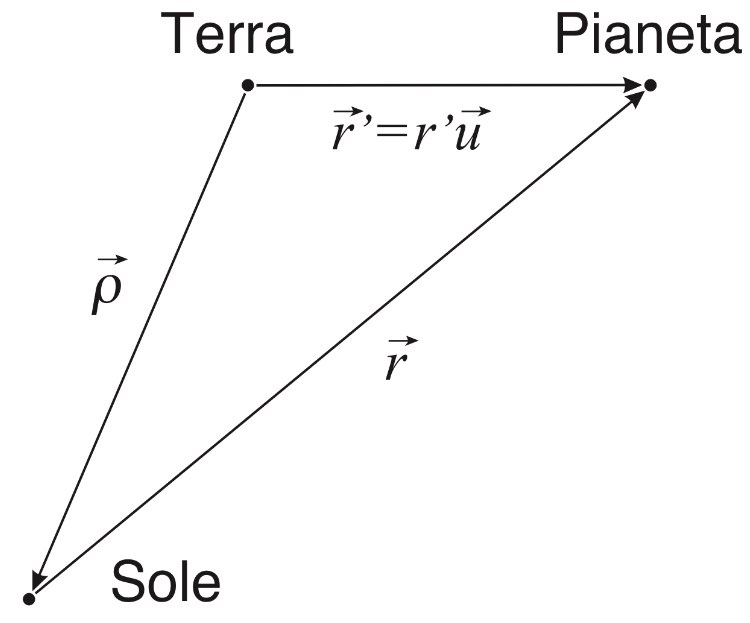
\includegraphics[width=\textwidth]{iterationorbit}

\end{figure}

\end{column}

\begin{column}{0.7\textwidth}

\begin{align*}
&\alpha_1=\alpha_1(i,\omega,\Omega,\chi,a,e,\phi_0;t_1)\\
&\delta_1=\delta_1(i,\omega,\Omega,\chi,a,e,\phi_0;t_1)\\
&\alpha_2=\alpha_2(i,\omega,\Omega,\chi,a,e,\phi_0;t_2)\\
&\delta_2=\delta_2(i,\omega,\Omega,\chi,a,e,\phi_0;t_2)\\
&\alpha_3=\alpha_3(i,\omega,\Omega,\chi,a,e,\phi_0;t_3)\\
&\delta_3=\delta_3(i,\omega,\Omega,\chi,a,e,\phi_0;t_3)
\end{align*}

\end{column}

\end{columns}

\begin{block}{Metodo iterativo}
da una soluzione approssimata ne ricaviamo una pi\'u corretta
\end{block}

\end{frame}

\subsection{Metodo di Laplace}




\subsection{Metodo di Gauss}

